%iffalse
\let\negmedspace\undefined
\let\negthickspace\undefined
\documentclass[journal,12pt,onecolumn]{IEEEtran}
\usepackage{cite}
\usepackage{amsmath,amssymb,amsfonts,amsthm}
\usepackage{algorithmic}
\usepackage{graphicx}
\usepackage{textcomp}
\usepackage{xcolor}
\usepackage{txfonts}
\usepackage{listings}
\usepackage{enumitem}
\usepackage{mathtools}
\usepackage{gensymb}
\usepackage{comment}
\usepackage[breaklinks=true]{hyperref}
\usepackage{tkz-euclide} 
\usepackage{listings}
\usepackage{gvv}                                        
%\def\inputGnumericTable{}                                 
\usepackage[latin1]{inputenc}                                
\usepackage{color}                                            
\usepackage{array}                                            
\usepackage{longtable}                                       
\usepackage{calc}                                             
\usepackage{multirow}                                         
\usepackage{hhline}                                           
\usepackage{ifthen}                                           
\usepackage{lscape}
\usepackage{tabularx}
\usepackage{array}
\usepackage{float}

\usepackage{enumitem}
\usepackage{xcolor}
%\usepackage{multicol}


\newtheorem{theorem}{Theorem}[section]
\newtheorem{problem}{Problem}
\newtheorem{proposition}{Proposition}[section]
\newtheorem{lemma}{Lemma}[section]
\newtheorem{corollary}[theorem]{Corollary}
\newtheorem{example}{Example}[section]
\newtheorem{definition}[problem]{Definition}
\newcommand{\BEQA}{\begin{eqnarray}}
\newcommand{\EEQA}{\end{eqnarray}}
\newcommand{\define}{\stackrel{\triangle}{=}}
\theoremstyle{remark}
\newtheorem{rem}{Remark}

\title{1.7.4}
\author{AI24BTECH11023 - Tarun Reddy Pakala}
\begin{document}
\bibliographystyle{IEEEtran}

\maketitle
\bigskip

\renewcommand{\thefigure}{\theenumi}
\renewcommand{\thetable}{\theenumi}


\textbf{Question}:\\
Using vectors, prove that the points \brak{2,-1,3},\brak{3,-5,1} and \brak{-1,11,9} are collinear.\\
\solution\\
\textbf{Step 1: Calculate the Vectors}

The vectors $\overrightarrow{AB}$ and $\overrightarrow{AC}$ are defined as follows:

$$
\overrightarrow{AB} = B - A = (3 - 2, -5 - (-1), 1 - 3) = (1, -4, -2)
$$

$$
\overrightarrow{AC} = C - A = (-1 - 2, 11 - (-1), 9 - 3) = (-3, 12, 6)
$$

\textbf{Step 2: Check for Parallelism}

Two vectors are parallel if one is a scalar multiple of the other. We need to determine if there exists a scalar $k$ such that:

$$
\overrightarrow{AC} = k \cdot \overrightarrow{AB}
$$

This gives us the following system of equations:

$$
(-3, 12, 6) = k(1, -4, -2)
$$

From the first component, we have:

$$
-3 = k \cdot 1 \quad \Rightarrow \quad k = -3
$$

From the second component:

$$
12 = k \cdot -4 \quad \Rightarrow \quad k = -3
$$

From the third component:

$$
6 = k \cdot -2 \quad \Rightarrow \quad k = -3
$$

Since we have $k = -3$ for all components, we conclude that:

$$
\overrightarrow{AC} = -3 \cdot \overrightarrow{AB}
$$

\textbf{Conclusion}

Since $\overrightarrow{AC}$ is a scalar multiple of $\overrightarrow{AB}$, the vectors are parallel. Therefore, the points $A$, $B$, and $C$ are collinear.

Thus, the points $(2, -1, 3)$, $(3, -5, 1)$, and $(-1, 11, 9)$ are indeed collinear.
\documentclass{article}
\usepackage{graphicx}

\begin{document}

\title{Figure on New Page Example}
\author{}
\date{}
\maketitle

% Some introductory text
This is some text that fills the page before the figure.

\newpage % Start a new page before the figure

\begin{figure}[h]
    \centering
    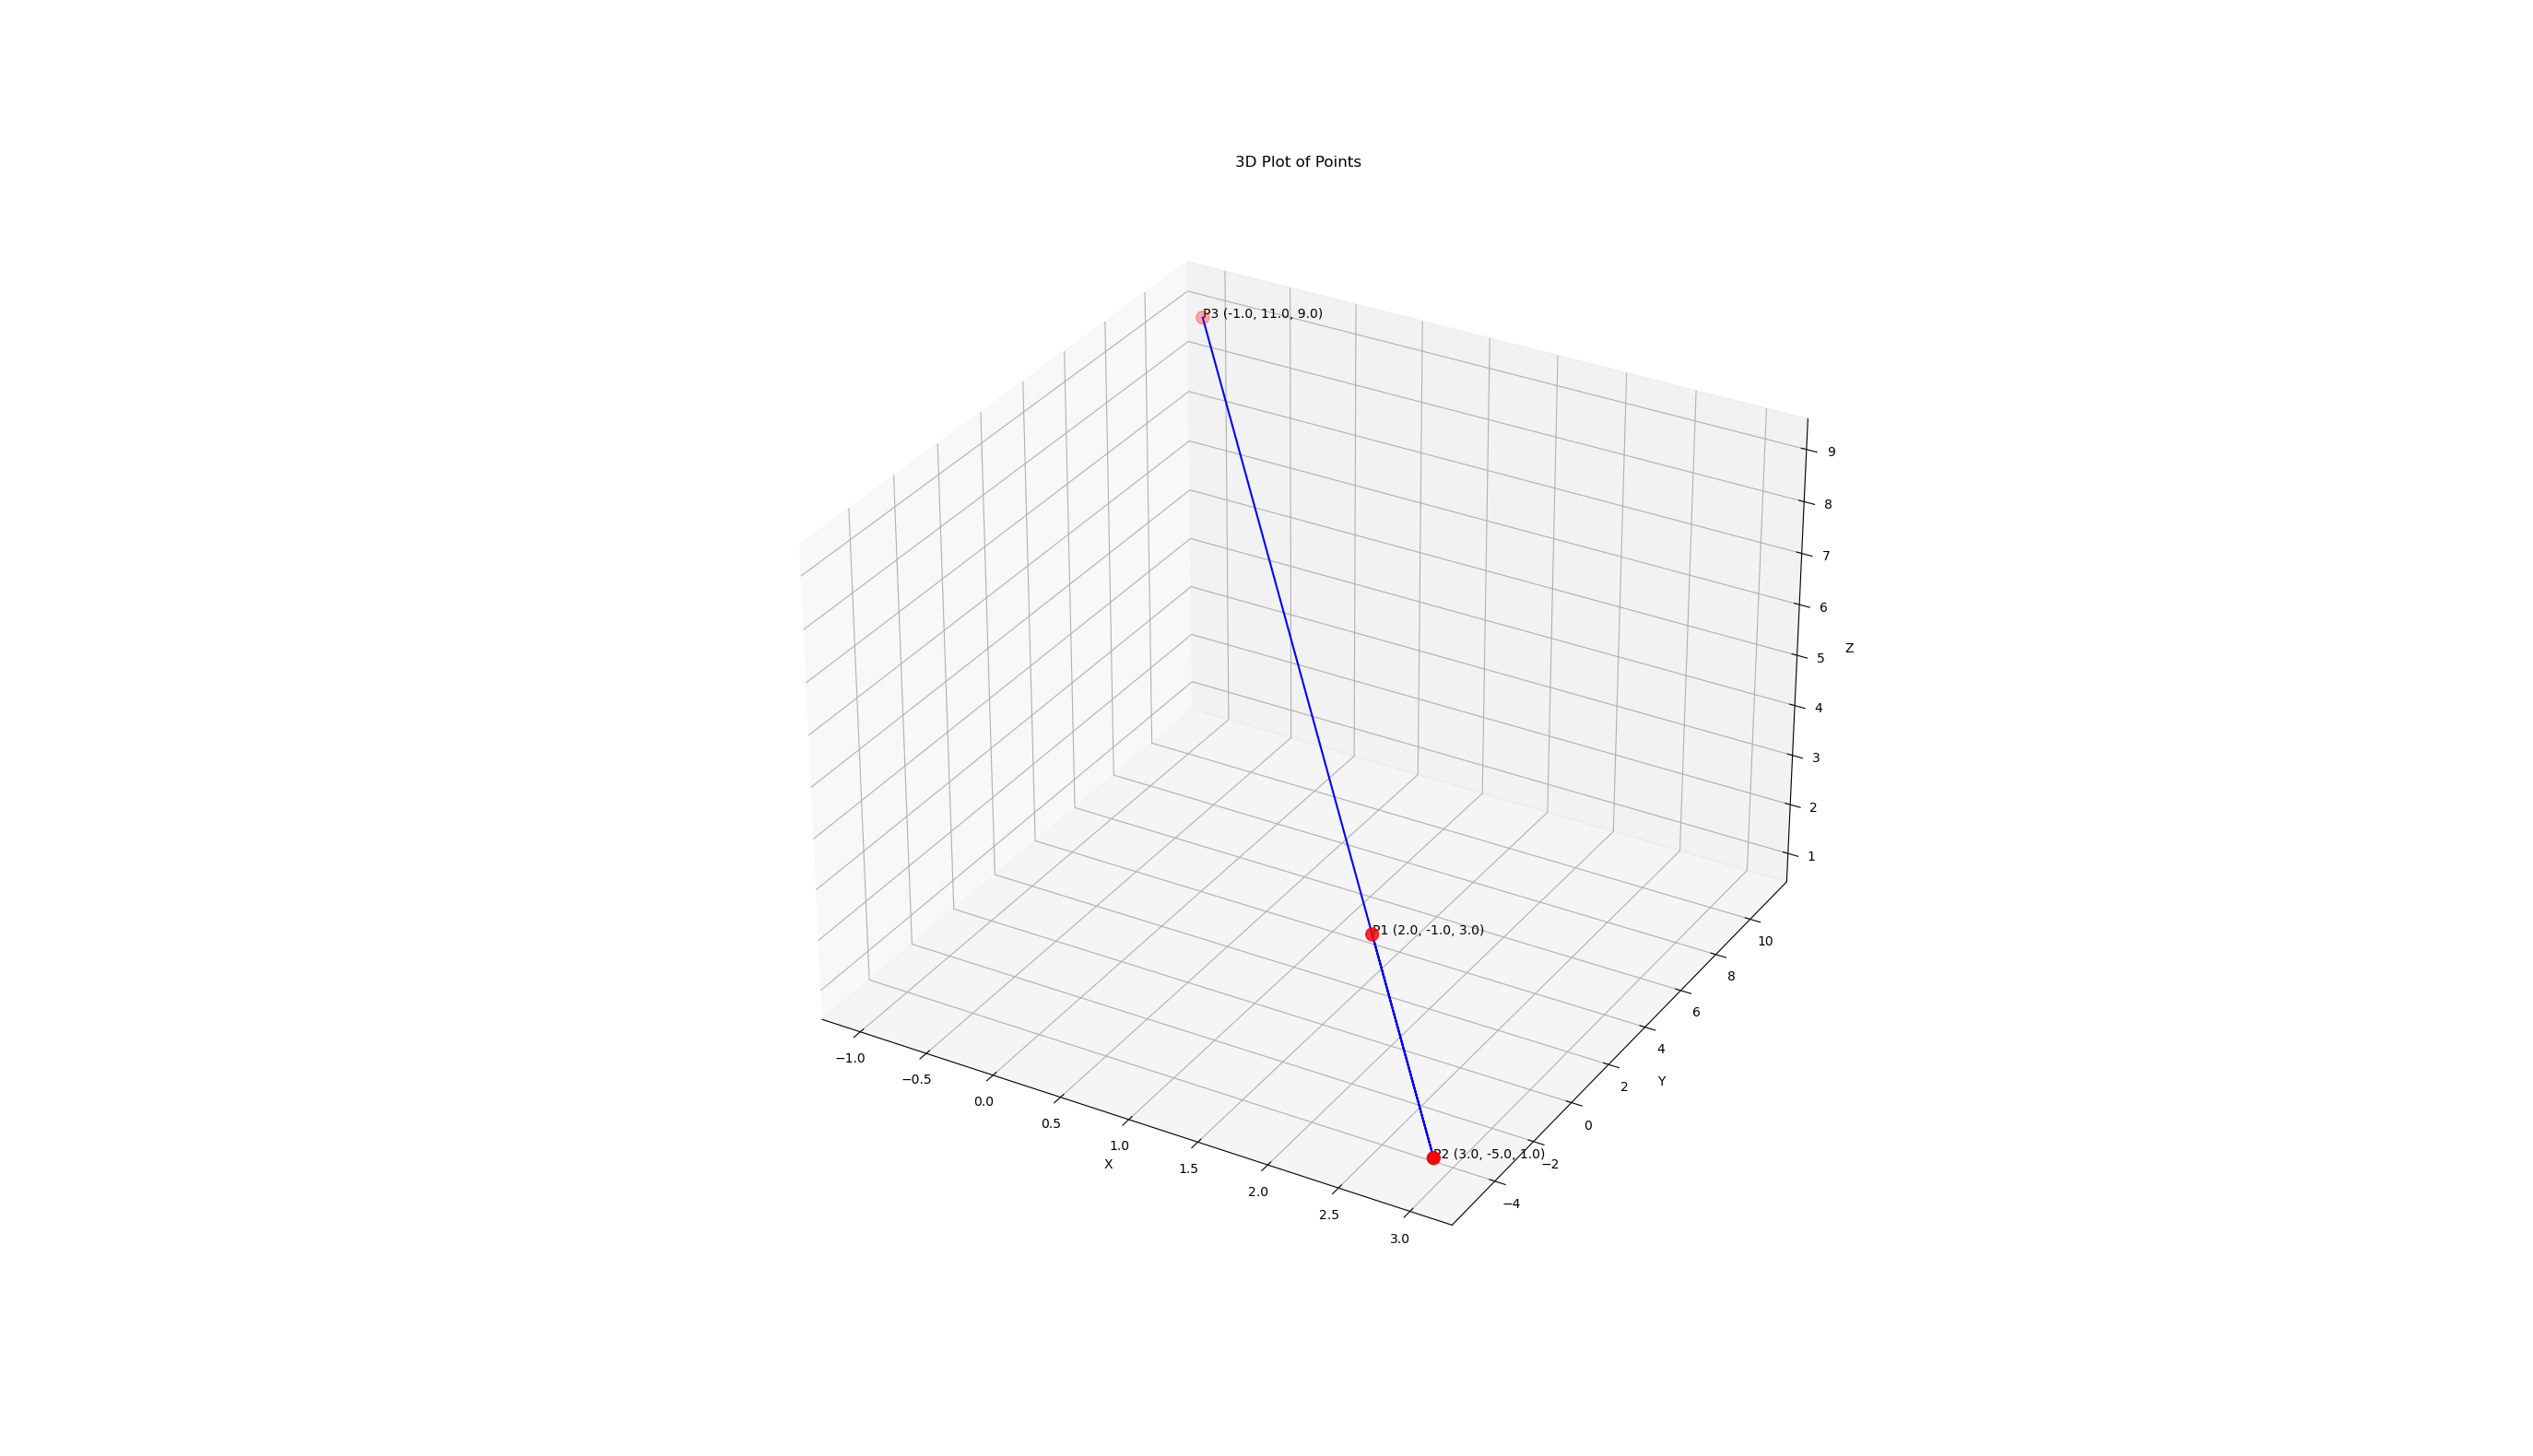
\includegraphics[width=\textwidth]{figure.png} 
    \label{fig:example_image}
\end{figure}

\end{document}
